\documentclass[aspectratio=169,t,xcolor=table]{beamer}
\usepackage[portuguese,brazilian,brazil]{babel}
\usepackage[utf8]{inputenc}

\usepackage{tikz}
\usepackage{booktabs} 
\usepackage{subcaption}
\usepackage{subfiles}

\usepackage{hyperref}
\usepackage{tabularx}
\usepackage{amsmath}
\usepackage{graphicx}
\usepackage{abntex2cite}
\usepackage{cite}
\usepackage{listings}


%\renewcommand\citeleft{[}
%\renewcommand\citeright{]}
\hypersetup{
	pdfborder={0 0 0},            
	pdftoolbar=true,            
	pdfmenubar=true,              
	pdffitwindow=false,
	pdfstartview={FitH},          
	pdfauthor={Erick, Pedro, Thiago, Vinicius, Daniel},
	pdftitle={Simulação Numérica do Problema de N-Corpos - Uma Análise Comparativa de Métodos de Runge-Kutta com Aplicação ao Sistema Solar}, 
	pdfsubject={Física, Sínteses e Aplicações}
	pdfproducer={LaTeX},   
	pdfcreator={pdfLaTeX},  
	pdfnewwindow=true,      
	colorlinks=true,      
	linkcolor=blue,          
	citecolor=blue,        
	filecolor=magenta,     
	urlcolor=blue
}
\usetheme{Ufg}


\setbeamertemplate{theorems}[numbered]
\setbeamertemplate{caption}[numbered]

\setPrimaryColor{UFGBlue} 
\setLogos{lib/logos/icmc.png}{lib/logos/licmc.png}




%_______________________________________________________________________________________________________________________
\begin{document}
	
	

%-------Capa-------	
%----------------------------------------------------------------------------------------------------------------------	
\title{Título a Definir}
\author{Erick Rodrigues Canterle\inst{1}  \and  Pedro Vinicius Souza Coimbra\inst{2} \and \\
	Thiago Ferreira de França e Queiroz\inst{3} \and Vinícius de Sá Ferreira \inst{4} \and \\
	Daniel Garcia Leal Raymundo\inst{5}}

\institute[USP] 
{
	\inst{1} \inst{2}\inst{3}\inst{4}
	ICMC - Instituto De Ciências Matemáticas e de Computação \\
	Universidade de São Paulo
	
	\inst{5}
	FCUP - Faculdade de Ciências da Universidade do Porto \\
	Universidade do Porto
}
\date{\today}
\frame[noframenumbering]{\titlepage}
%----------------------------------------------------------------------------------------------------------------------



%-------Sumário-------	
%----------------------------------------------------------------------------------------------------------------------	
\setLayout{vertical}
\begin{frame}{Índices}
	\tableofcontents
\end{frame}
%----------------------------------------------------------------------------------------------------------------------



%-------Introdução-------	
%----------------------------------------------------------------------------------------------------------------------	
\section{Introdução}

\setLayout{mainpoint}
\begin{frame}
	\frametitle{Introdução}
\end{frame}


\setLayout{vertical}
\begin{frame}{}
	\smaller
	\begin{block}{O que é \textit{HgFlow/HigThree}?}
		\vspace{0.25 cm}
		O \textit{HigFlow/HigTree} é uma biblioteca desenvolvida majoritariamente em C, que disponibiliza um conjunto de ferramentas voltadas à realização de simulações numéricas em domínios complexos. Esses domínios são discretizados por meio de uma estrutura de dados de malha cartesiana baseada em árvores generalizadas, denominada \textbf{HiG-Tree}. A biblioteca foi projetada com foco no paralelismo, empregando o padrão \textbf{MPI} (Message Passing Interface)\textbf{ / Zoltan} para a distribuição de dados e da carga computacional.
	\end{block}
	
	\begin{block}{Um pouco de História}
		\vspace{0.25 cm}
		
		Esta biblioteca foi desenvolvida em (informar data) sob a supervisão do professor Antonio Castelo Filho e \textbf{CIA}, com financiamento da Petrobras. O projeto contou com a colaboração de mais de dez alunos de pós-graduação, que contribuíram para seu aprimoramento e aplicação em diversas pesquisas, resultando na publicação de inúmeros artigos científicos, como  \citeauthor{Sousa2019}, \citeauthor{CastilloSanchez2023} e dissertações como \citeauthor{raymundo}.
	\end{block}
\end{frame}

\begin{frame}{\smaller \smaller Dimensão do Projeto}
	
	\begin{figure}
		\vspace{-0.3cm}
		\centering
		\caption{\smaller Escopo do projeto (disponível em: \url{https://github.com/antoniocastelofilho/HigFlow}) mensurado pela quantidade de arquivos e pelo total de linhas de código.}
		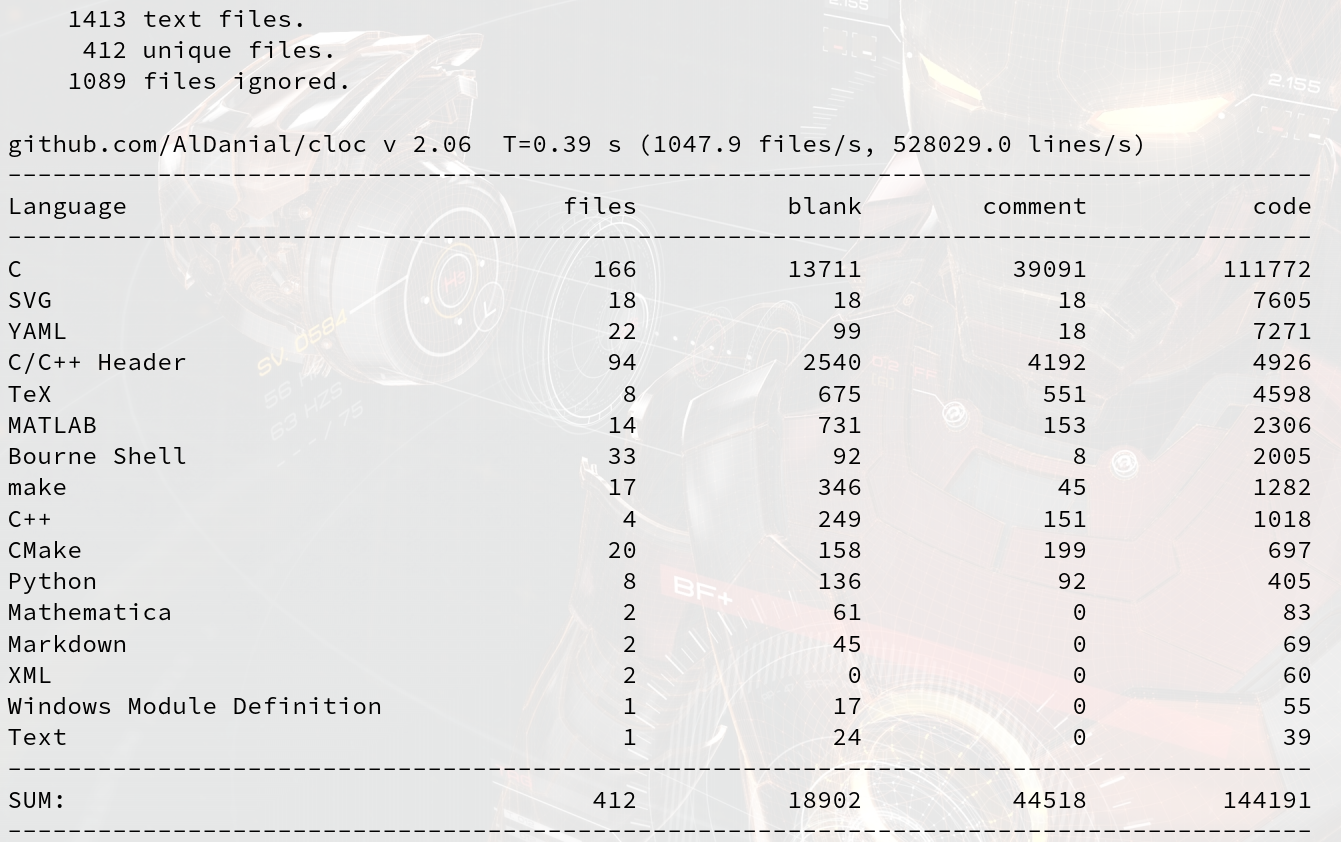
\includegraphics[height=0.7\textheight]{imgs/dimencao_do_projeto.png}
	\end{figure}
\end{frame}


%----------------------------------------------------------------------------------------------------------------------





%_______________________________________________________________________________________________________________________
% Estrutura de dados da HiGtree
\subfile{../vinicius/vinicius.tex}

 % WLS e Stencil
\subfile{../pedro/pedro.tex} 

% Paralelismo e fringes
\subfile{../thiago/thiago.tex} 

% Exemplo Poisson
\subfile{../erick/erick.tex} 
%_______________________________________________________________________________________________________________________




%-------Agradecimentos-------	
%----------------------------------------------------------------------------------------------------------------------
\section{Agradecimentos}


\setLayout{blank}
\begin{frame}
	
	\centering
	
	\vspace{1cm}
	\textbf{Nossos sinceros agradecimentos ao Daniel. Sua ajuda foi indispensável para a  para a realização deste trabalho}
	
	\vspace{5cm}
	

	\begin{figure}
		\centering
		\begin{subfigure}{0.2\textwidth}
			\centering
			
\includegraphics[height=1cm]{lib/logos/icmc.png}
		\end{subfigure}
		\qquad 
		\begin{subfigure}{0.2\textwidth}
			\centering
			
\includegraphics[height=1cm]{lib/logos/logo_usp_white.png}
		\end{subfigure}
		
	\end{figure}
	
\end{frame}



\setLayout{blank}
\begin{frame}
	
	\centering
	\vspace{2cm}
	
	\textbf{\Huge Muito Obrigado Pela Atenção}
	
	\ \\
	
	\textbf{Dúvidas e Sugestões}
	\ \\
	
	\text{\footnotesize Erick Rodrigues Canterle, } \\
	\text{\footnotesize pedro.coimbra@usp.br,} \\
	\text{\footnotesize queiroztff@usp.br ou} \\
	\text{\footnotesize desaferreirav@usp.br}
	\vspace{2cm}
	\begin{figure}
		\centering
		\begin{subfigure}{0.2\textwidth}
			\centering
			
\includegraphics[height=1cm]{lib/logos/icmc.png}
		\end{subfigure}
		\qquad 
		\begin{subfigure}{0.2\textwidth}
			\centering
			
\includegraphics[height=1cm]{lib/logos/logo_usp_white.png}
		\end{subfigure}
		
	\end{figure}
	
\end{frame}
%----------------------------------------------------------------------------------------------------------------------



%-------Referências-------	
%----------------------------------------------------------------------------------------------------------------------
\section{Referências}
\setLayout{horizontal}
\begin{frame}[allowframebreaks]
	\frametitle{Referências}
	\smaller
	\bibliography{../references.bib}
	\nocite{}
	\bibliographystyle{abntex2-alf}
\end{frame}
%----------------------------------------------------------------------------------------------------------------------	




\end{document}
%_______________________________________________________________________________________________________________________